%%%%%%%%%%%%%%%%%%%%%%%%%%%%%%%%%%%%%%%%%%%%%%%%%%%%%%%%%%%%%%%%
%
%  Template for homework of Introduction to Machine Learning.
%
%  Fill in your name, lecture number, lecture date and body
%  of homework as indicated below.
%         
%%%%%%%%%%%%%%%%%%%%%%%%%%%%%%%%%%%%%%%%%%%%%%%%%%%%%%%%%%%%%%%%
\documentclass[11pt,letter,notitlepage]{article}
%Mise en page
\usepackage[left=2cm, right=2cm, lines=45, top=0.8in, bottom=0.7in]{geometry}
\usepackage{fancyhdr}
\usepackage{fancybox}
\usepackage{graphicx}
\usepackage{pdfpages}
\usepackage{enumitem}
\usepackage{algorithm}
\usepackage{algorithmic}
\usepackage{pifont}
\renewcommand{\headrulewidth}{1.5pt}
\renewcommand{\footrulewidth}{1.5pt}
\newcommand\Loadedframemethod{TikZ}
\usepackage[framemethod=\Loadedframemethod]{mdframed}
\usepackage{amssymb,amsmath}
\usepackage{extarrows}
\usepackage{amsthm}
\usepackage{thmtools}
\usepackage{bm}
\usepackage{pifont}
\usepackage{listings}
\usepackage{xcolor}

\lstset{
    language=Python,
    basicstyle=\ttfamily\small,
    keywordstyle=\color{blue},
    commentstyle=\color{teal},
    stringstyle=\color{red},
    showstringspaces=false,
    breaklines=true,
    frame=single
}

\setlength{\topmargin}{0pt}
\setlength{\textheight}{9in}
\setlength{\headheight}{0pt}
\setlength{\oddsidemargin}{0.25in}
\setlength{\textwidth}{6in}
%%%%%%%%%%%%%%%%%%%%%%%%
%%%%%% Define math operator %%%%%
%%%%%%%%%%%%%%%%%%%%%%%%
\DeclareMathOperator*{\argmin}{\bf argmin}
\DeclareMathOperator*{\relint}{\bf relint\,}
\DeclareMathOperator*{\dom}{\bf dom\,}
\DeclareMathOperator*{\intp}{\bf int\,}
%%%%%%%%%%%%%%%%%%%%%%%
\setlength{\topmargin}{0pt}
\setlength{\textheight}{9in}
\setlength{\headheight}{0pt}
\setlength{\oddsidemargin}{0.25in}
\setlength{\textwidth}{6in}
\pagestyle{fancy}
%%%%%%%%%%%%%%%%%%%%%%%%
%% Define the Exercise environment %%
%%%%%%%%%%%%%%%%%%%%%%%%
\mdtheorem[
topline=false,
rightline=false,
leftline=false,
bottomline=false,
leftmargin=-10,
rightmargin=-10
]{exercise}{\textbf{Exercise}}
\renewcommand{\theexercise}{\arabic{exercise}:}
%%%%%%%%%%%%%%%%%%%%%%%
%% End of the Exercise environment %%
%%%%%%%%%%%%%%%%%%%%%%%
%%%%%%%%%%%%%%%%%%%%%%%%
%% Define the Problem environment %%
%%%%%%%%%%%%%%%%%%%%%%%%
\mdtheorem[
topline=false,
rightline=false,
leftline=false,
bottomline=false,
leftmargin=-10,
rightmargin=-10
]{problem}{\textbf{Problem}}
%%%%%%%%%%%%%%%%%%%%%%%
%% End of the Exercise environment %%
%%%%%%%%%%%%%%%%%%%%%%%
%%%%%%%%%%%%%%%%%%%%%%%
%% Define the Solution Environment %%
%%%%%%%%%%%%%%%%%%%%%%%
\declaretheoremstyle
[
spaceabove=0pt,
spacebelow=0pt,
headfont=\normalfont\bfseries,
notefont=\mdseries,
notebraces={(}{)},
headpunct={:},
headindent={},
postheadspace=\newline,
bodyfont=\normalfont,
qed=$\blacksquare$,
preheadhook={\begin{mdframed}[style=myframedstyle]},
postfoothook=\end{mdframed},
]{mystyle}
\declaretheorem[style=mystyle,title=Solution]{solution}
\mdfdefinestyle{myframedstyle}{%
	topline=false,
	rightline=false,
	leftline=false,
	bottomline=false,
	skipabove=-6ex,
	leftmargin=-10,
	rightmargin=-10,
	backgroundcolor=black!5}
%%%%%%%%%%%%%%%%%%%%%%%
%% End of the Solution environment

\renewcommand{\eqref}[1]{Eq.~(\ref{#1})}
\newcommand{\figref}[1]{Fig.~\ref{#1}}


\newcommand{\proj}[2]{\textbf{P}_{#2} (#1)}
\newcommand{\lspan}[1]{\textbf{span}  (#1)  }
\newcommand{\rank}[1]{ \textbf{rank}  (#1)  }
\newcommand{\tr}{ \operatorname{tr}  }
\newcommand{\RNum}[1]{\uppercase\expandafter{\romannumeral #1\relax}}

\newcommand{\mb}[1]{\mathbf{#1}}

\DeclareMathOperator*{\cl}{\bf cl\,}
\DeclareMathOperator*{\bd}{\bf bd\,}
\DeclareMathOperator*{\conv}{\bf conv\,}
\DeclareMathOperator*{\epi}{\bf epi\,}

% Definition environment	
\theoremstyle{definition}	
\newtheorem{definition}{Definition}	


%%%%%%%%%%%%%%%%%%%%%%%%%%%%%%%%%%%%%%%%%%
%%           Homework info.             %%
\newcommand{\posted}{\text{Mar. 23rd, 2025}}       			%%% FILL IN POST DATE HERE
\newcommand{\due}{\text{Apr. 6th, 2025}} 			%%% FILL IN Due DATE HERE
\newcommand{\hwno}{\text{2}} 		           			%%% FILL IN LECTURE NUMBER HERE
%%%%%%%%%%%%%%%%%%%%%%%%%%%%%%%%%%%%%%%%%%

%%%%%%%%%%%%%%%%%%%%%%%%%%%%%%%%%%%%
%%    Put your information here   %%
\newcommand{\name}{\text{Jinghao Chen}}  	          			%%% FILL IN YOUR NAME HERE
\newcommand{\id}{\text{PB23010359}}		       			%%% FILL IN YOUR ID HERE
%%%%%%%%%%%%%%%%%%%%%%%%%%%%%%%%%%%%

\lhead{
 	\textbf{\name}
}
\rhead{
 	\textbf{\id}
}
\chead{\textbf{
		Homework \hwno
}}


\begin{document}
	\vspace*{-4\baselineskip}
	\thispagestyle{empty}
	
	
	\begin{center}
		{\bf\large Introduction to Optimization}\\
		{Spring 2026}\\
		University of Science and Technology of China
	\end{center}
	
	\noindent
	Lecturer: Nick  			 %%% FILL IN LECTURER HERE
	\hfill
	Homework \hwno             			
	\\
	Posted: \posted
	\hfill
	Due: \due
    \\
	Name: \name             			
	\hfill
	ID: \id
	
	\noindent
	\rule{\textwidth}{2pt}
	
	\medskip
	
	
	
	
	
	%%%%%%%%%%%%%%%%%%%%%%%%%%%%%%%%%%%%%%%%%%%%%%%%%%%%%%%%%%%%%%%%
	%% BODY OF HOMEWORK GOES HERE
	%%%%%%%%%%%%%%%%%%%%%%%%%%%%%%%%%%%%%%%%%%%%%%%%%%%%%%%%%%%%%%%%

\begin{exercise}
For all possible cases of $P \in \mathbb{S}^d$, $q \in \mathbb{R}^d$:
\[
\begin{aligned}
\text{minimize} \quad & x^T P x + q^T x
\end{aligned}
\]
\end{exercise}

\newpage

\begin{solution}
Let
\[
f(x)=x^TPx+q^Tx,\qquad P\in\mathbb S^d,\ q\in\mathbb R^d.
\]
Since \(P=P^T\), we classify all cases by the sign of \(P\).

\[
\nabla f(x)=2Px+q.
\]

\ding{172}\ \textbf{If \(P\not\succeq 0\).}

Then \(\exists\,v\neq 0\) such that
\[
v^TPv<0.
\]
Take \(x=t v\). Then
\[
f(tv)=t^2v^TPv+tq^Tv.
\]
Hence
\[
t\to\infty
\quad\Longrightarrow\quad
f(tv)\to -\infty.
\]
Therefore,
\[
\inf_{x\in\mathbb R^d} f(x)=-\infty.
\]

\ding{173}\ \textbf{If \(P\succeq 0\) and \(q\notin\mathrm{Range}(P)\).}

Since \(P=P^T\),
\[
\mathrm{Range}(P)=\mathrm{Null}(P)^\perp.
\]
Thus
\[
q\notin\mathrm{Range}(P)
\quad\Longrightarrow\quad
\exists\,z\in\mathrm{Null}(P)\ \text{such that}\ q^Tz\neq 0.
\]
Because \(Pz=0\),
\[
f(x+t z)
=(x+t z)^TP(x+t z)+q^T(x+t z)
= x^TPx+q^Tx+t\,q^Tz.
\]
Choose the sign of \(t\) so that \(tq^Tz\to -\infty\). Then
\[
\inf_{x\in\mathbb R^d} f(x)=-\infty.
\]

\ding{174}\ \textbf{If \(P\succeq 0\) and \(q\in\mathrm{Range}(P)\).}

Then
\[
2Px+q=0
\]
has a solution. Let \(x_0\) satisfy
\[
2Px_0+q=0.
\]
Then
\[
q=-2Px_0,
\]
and for any \(x\in\mathbb R^d\),
\[
\begin{aligned}
f(x)-f(x_0)
&=x^TPx+q^Tx-\bigl(x_0^TPx_0+q^Tx_0\bigr)\\
&=x^TPx-2x_0^TPx-x_0^TPx_0+2x_0^TPx_0\\
&=x^TPx-2x_0^TPx+x_0^TPx_0\\
&=(x-x_0)^TP(x-x_0)\ge 0.
\end{aligned}
\]
Hence \(x_0\) is a minimizer.

Moreover,
\[
2Px+q=0
\quad\Longleftrightarrow\quad
P(x-x_0)=0
\quad\Longleftrightarrow\quad
x-x_0\in\mathrm{Null}(P).
\]
So the set of minimizers is
\[
\arg\min f
=
\{x:2Px+q=0\}
=
x_0+\mathrm{Null}(P).
\]

If \(P^\dagger\) is the Moore--Penrose pseudoinverse, one minimizer is
\[
x^\star=-\frac12 P^\dagger q,
\]
and
\[
\arg\min f
=
-\frac12 P^\dagger q+\mathrm{Null}(P).
\]
The optimal value is
\[
f^\star=-\frac14 q^TP^\dagger q.
\]

Therefore,
\[
\boxed{
\begin{array}{ll}
\ding{172}\ \text{If }P\not\succeq 0, & \inf f(x)=-\infty.\\[0.4em]
\ding{173}\ \text{If }P\succeq 0,\ q\notin\mathrm{Range}(P), & \inf f(x)=-\infty.\\[0.4em]
\ding{174}\ \text{If }P\succeq 0,\ q\in\mathrm{Range}(P), &
\arg\min f=\{x:2Px+q=0\}.
\end{array}}
\]

In particular, if \(P\succ 0\), then
\[
x^\star=-\frac12 P^{-1}q,
\qquad
f^\star=-\frac14 q^TP^{-1}q,
\]
and the minimizer is unique.

If \(P=0\), then
\[
f(x)=q^Tx.
\]
Thus
\[
q=0 \Longrightarrow \text{every }x\text{ is optimal},
\qquad
q\neq 0 \Longrightarrow \inf f(x)=-\infty.
\]
\end{solution}

\newpage

\begin{exercise}
\textit{Some simple LPs}. Give an explicit solution of each of the following LPs.

\begin{enumerate}[label=(\alph*)]
    \item \textit{Minimizing a linear function over an affine set.}
    \[
    \begin{aligned}
    \text{minimize} \quad & c^T x \\
    \text{subject to} \quad & Ax=b.
    \end{aligned}
    \]

    \item \textit{Minimizing a linear function over a halfspace.}
    \[
    \begin{aligned}
    \text{minimize} \quad & c^T x \\
    \text{subject to} \quad & a^T x \le b,
    \end{aligned}
    \]
    where $a \ne 0$.

    \item \textit{Minimizing a linear function over a rectangle.}
    \[
    \begin{aligned}
    \text{minimize} \quad & c^T x \\
    \text{subject to} \quad & l \preceq x \preceq u,
    \end{aligned}
    \]
    where $l$ and $u$ satisfy $l \preceq u$.

    \item \textit{Minimizing a linear function over the probability simplex.}
    \[
    \begin{aligned}
    \text{minimize} \quad & c^T x \\
    \text{subject to} \quad & \mathbf{1}^T x = 1,\quad x \succeq 0.
    \end{aligned}
    \]

    What happens if the equality constraint is replaced by an inequality
    $\mathbf{1}^T x \le 1$?

    We can interpret this LP as a simple portfolio optimization problem.
    The vector $x$ represents the allocation of our total budget over different assets,
    with $x_i$ the fraction invested in asset $i$. The return of each investment is fixed
    and given by $-c_i$, so our total return (which we want to maximize) is $-c^T x$.
    If we replace the budget constraint $\mathbf{1}^T x = 1$ with an inequality
    $\mathbf{1}^T x \le 1$, we have the option of not investing a portion of the total budget.
\end{enumerate}
\end{exercise}

\newpage

\begin{solution}
\leavevmode\vspace{-2em}
\begin{enumerate}[label=(\alph*)]

\item
Let \(F=\{x:Ax=b\}\).

\ding{172}\ \textbf{If \(b\notin\mathrm{Range}(A)\).}

Then \(F=\varnothing\). Hence the LP is infeasible.

\ding{173}\ \textbf{If \(b\in\mathrm{Range}(A)\) and \(c\in\mathrm{Range}(A^T)\).}

Take any \(x_0\) such that
\[
Ax_0=b.
\]
Then every feasible point can be written as
\[
x=x_0+z,\qquad z\in\mathrm{Null}(A).
\]
Since \(c\in\mathrm{Range}(A^T)=\mathrm{Null}(A)^\perp\),
\[
c^Tz=0,\qquad \forall z\in\mathrm{Null}(A).
\]
Therefore,
\[
c^Tx=c^Tx_0,\qquad \forall x\in F.
\]
So every feasible point is optimal:
\[
\arg\min c^Tx = \{x:Ax=b\}.
\]

\ding{174}\ \textbf{If \(b\in\mathrm{Range}(A)\) and \(c\notin\mathrm{Range}(A^T)\).}

Then
\[
c\notin\mathrm{Null}(A)^\perp
\quad\Longrightarrow\quad
\exists\,z\in\mathrm{Null}(A)\ \text{such that}\ c^Tz\neq 0.
\]
Take any feasible \(x_0\). Since \(A(x_0+t z)=b\),
\[
c^T(x_0+t z)=c^Tx_0+t\,c^Tz.
\]
Choose the sign of \(t\) so that \(t\,c^Tz\to -\infty\). Hence
\[
\inf c^Tx=-\infty.
\]

\medskip

\item
\ding{172}\ \textbf{If \(c\notin -\mathbb R_+ a\).}

Then \(\exists\,d\) such that
\[
a^Td=0,\qquad c^Td<0.
\]
Take any feasible \(x_0\), i.e. \(a^Tx_0\le b\). Then
\[
a^T(x_0+t d)=a^Tx_0\le b,\qquad \forall t\ge 0,
\]
so \(x_0+t d\) is feasible for all \(t\ge 0\). But
\[
c^T(x_0+t d)=c^Tx_0+t\,c^Td\to -\infty.
\]
Hence
\[
\inf c^Tx=-\infty.
\]

\ding{173}\ \textbf{If \(c=-\lambda a\) for some \(\lambda\ge 0\).}

Then
\[
c^Tx=-\lambda a^Tx.
\]

If \(\lambda=0\), then \(c=0\), and every feasible point is optimal.

If \(\lambda>0\), then
\[
a^Tx\le b
\quad\Longrightarrow\quad
c^Tx=-\lambda a^Tx\ge -\lambda b.
\]
Equality holds iff
\[
a^Tx=b.
\]
Therefore,
\[
p^\star=-\lambda b,
\qquad
\arg\min c^Tx=\{x:a^Tx=b\}.
\]

\medskip

\item
Since
\[
c^Tx=\sum_{i=1}^n c_i x_i,
\qquad
l_i\le x_i\le u_i,
\]
the problem separates coordinatewise.

For each \(i\),
\[
x_i^\star=
\begin{cases}
l_i, & c_i>0,\\[0.3em]
u_i, & c_i<0,\\[0.3em]
\text{any value in }[l_i,u_i], & c_i=0.
\end{cases}
\]
Hence
\[
\arg\min c^Tx
=
\left\{
x:
x_i=
\begin{cases}
l_i, & c_i>0,\\
u_i, & c_i<0,\\
\text{any }x_i\in[l_i,u_i], & c_i=0
\end{cases}
\right\}.
\]
The optimal value is
\[
p^\star=\sum_{i=1}^n
\begin{cases}
c_i l_i, & c_i>0,\\
c_i u_i, & c_i<0,\\
0, & c_i=0.
\end{cases}
\]

\medskip

\item
Let
\[
m=\min_i c_i,
\qquad
I=\{i:c_i=m\}.
\]

If
\[
\mathbf 1^Tx=1,\qquad x\succeq 0,
\]
then
\[
c^Tx=\sum_{i=1}^n c_i x_i \ge \sum_{i=1}^n m x_i=m\sum_{i=1}^n x_i=m.
\]
Equality holds iff
\[
x_i=0,\qquad \forall i\notin I.
\]
Therefore,
\[
p^\star=m,
\]
and
\[
\arg\min c^Tx
=
\left\{
x:
\mathbf 1^Tx=1,\ x\succeq 0,\ x_i=0\ \forall i\notin I
\right\}.
\]
In particular, any \(e_j\) with \(j\in I\) is optimal.

Now replace \(\mathbf 1^Tx=1\) by
\[
\mathbf 1^Tx\le 1,\qquad x\succeq 0.
\]

\ding{172}\ \textbf{If \(m<0\).}

Then it is optimal to invest the whole budget in the assets with smallest \(c_i\):
\[
p^\star=m,
\]
and
\[
\arg\min c^Tx
=
\left\{
x:
\mathbf 1^Tx=1,\ x\succeq 0,\ x_i=0\ \forall i\notin I
\right\}.
\]

\ding{173}\ \textbf{If \(m=0\).}

Then
\[
c^Tx\ge 0,
\]
and equality holds iff
\[
x_i=0,\qquad \forall i\notin I.
\]
Hence
\[
p^\star=0,
\]
and
\[
\arg\min c^Tx
=
\left\{
x:
\mathbf 1^Tx\le 1,\ x\succeq 0,\ x_i=0\ \forall i\notin I
\right\}.
\]

\ding{174}\ \textbf{If \(m>0\).}

Then for every \(x\succeq 0\),
\[
c^Tx\ge 0,
\]
and equality holds only at
\[
x=0.
\]
Thus
\[
p^\star=0,
\qquad
x^\star=0.
\]

\end{enumerate}

\end{solution}

\newpage

\begin{exercise}
\textit{Some simple QCQPs}. Give an explicit solution of each of the following QCQPs.

\begin{enumerate}[label=(\alph*)]
    \item \textit{Minimizing a linear function over an ellipsoid centered at the origin.}
    \[
    \begin{aligned}
    \text{minimize} \quad & c^T x \\
    \text{subject to} \quad & x^T A x \le 1,
    \end{aligned}
    \]
    where $A \in \mathbb{S}_{++}^n$ and $c \ne 0$.
    What is the solution if the problem is not convex
    ($A \notin \mathbb{S}_{+}^n$)?

    \item \textit{Minimizing a linear function over an ellipsoid.}
    \[
    \begin{aligned}
    \text{minimize} \quad & c^T x \\
    \text{subject to} \quad & (x-x_c)^T A (x-x_c) \le 1,
    \end{aligned}
    \]
    where $A \in \mathbb{S}_{++}^n$ and $c \ne 0$.

    \item \textit{Minimizing a quadratic form over an ellipsoid centered at the origin.}
    \[
    \begin{aligned}
    \text{minimize} \quad & x^T B x \\
    \text{subject to} \quad & x^T A x \le 1,
    \end{aligned}
    \]
    where $A \in \mathbb{S}_{++}^n$ and $B \in \mathbb{S}_{+}^n$.
    Also consider the nonconvex extension with $B \notin \mathbb{S}_{+}^n$.
    (See \S B.1.)
\end{enumerate}

\vspace{0.5em}
\noindent\textbf{Reference B.1.} \textbf{Single constraint quadratic optimization.}

We consider the problem with one constraint
\[
\begin{aligned}
\text{minimize} \quad & x^T A_0 x + 2b_0^T x + c_0 \\
\text{subject to} \quad & x^T A_1 x + 2b_1^T x + c_1 \le 0,
\end{aligned}
\tag{B.1}
\]
with variable $x \in \mathbb{R}^n$, and problem parameters
$A_i \in \mathbb{S}^n$, $b_i \in \mathbb{R}^n$, $c_i \in \mathbb{R}$.
We do not assume that $A_i \succeq 0$, so problem (B.1) is not a convex optimization problem.
\end{exercise}

\newpage

\begin{solution}
\leavevmode\vspace{-2em}
\begin{enumerate}[label=(\alph*)]

\item
Consider
\[
\begin{aligned}
\text{minimize}\quad & c^T x\\
\text{subject to}\quad & x^T A x\le 1,
\end{aligned}
\qquad A\in\mathbb S_{++}^n,\ c\neq 0.
\]

Since \(A\succ 0\),
\[
c^T x
=
(A^{-1/2}c)^T(A^{1/2}x)
\ge
-\|A^{-1/2}c\|_2\,\|A^{1/2}x\|_2.
\]
Also,
\[
x^T A x\le 1
\quad\Longrightarrow\quad
\|A^{1/2}x\|_2\le 1.
\]
Hence
\[
c^T x\ge -\|A^{-1/2}c\|_2
= -\sqrt{c^T A^{-1}c}.
\]
Equality holds when
\[
A^{1/2}x
=
-\frac{A^{-1/2}c}{\|A^{-1/2}c\|_2},
\]
i.e.,
\[
x^\star
=
-\frac{A^{-1}c}{\sqrt{c^T A^{-1}c}}.
\]
Therefore,
\[
p^\star=-\sqrt{c^T A^{-1}c},
\qquad
x^\star
=
-\frac{A^{-1}c}{\sqrt{c^T A^{-1}c}}.
\]

\medskip

Now consider \(A\notin\mathbb S_+^n\).

Then \(\exists\,v\neq 0\) such that
\[
v^TAv<0.
\]

\ding{172}\ \textbf{If \(c^Tv\neq 0\).}

Choose the sign of \(v\) so that
\[
c^Tv<0.
\]
Then for any \(t>0\),
\[
(tv)^T A (tv)=t^2 v^TAv\le 1,
\]
so \(tv\) is feasible, and
\[
c^T(tv)=t\,c^Tv\to -\infty.
\]
Hence
\[
\inf c^T x=-\infty.
\]

\ding{173}\ \textbf{If \(c^Tv=0\).}

Let
\[
d=-c+t v.
\]
Then
\[
c^T d=-\|c\|_2^2<0.
\]
Moreover,
\[
d^T A d
=
c^T A c-2t\,c^TAv+t^2 v^TAv.
\]
Since \(v^TAv<0\), for \(t\) large enough,
\[
d^TAd<0.
\]
Hence for any \(\alpha>0\),
\[
(\alpha d)^T A (\alpha d)=\alpha^2 d^TAd\le 1,
\]
so \(\alpha d\) is feasible, and
\[
c^T(\alpha d)=\alpha\, c^Td\to -\infty.
\]
Thus
\[
\inf c^T x=-\infty.
\]

Therefore, if \(A\notin\mathbb S_+^n\), the problem is unbounded below.

\medskip

\item
Consider
\[
\begin{aligned}
\text{minimize}\quad & c^T x\\
\text{subject to}\quad & (x-x_c)^T A (x-x_c)\le 1,
\end{aligned}
\qquad A\in\mathbb S_{++}^n,\ c\neq 0.
\]

Let
\[
y=x-x_c.
\]
Then the problem becomes
\[
\begin{aligned}
\text{minimize}\quad & c^T(y+x_c)=c^Ty+c^Tx_c\\
\text{subject to}\quad & y^T A y\le 1.
\end{aligned}
\]
By part (a),
\[
y^\star=-\frac{A^{-1}c}{\sqrt{c^T A^{-1}c}}.
\]
Hence
\[
x^\star
=
x_c-\frac{A^{-1}c}{\sqrt{c^T A^{-1}c}},
\]
and
\[
p^\star
=
c^T x_c-\sqrt{c^T A^{-1}c}.
\]

\medskip

\item
Consider
\[
\begin{aligned}
\text{minimize}\quad & x^T B x\\
\text{subject to}\quad & x^T A x\le 1,
\end{aligned}
\qquad A\in\mathbb S_{++}^n.
\]

Let
\[
y=A^{1/2}x,
\qquad
C=A^{-1/2}BA^{-1/2}.
\]
Then
\[
x=A^{-1/2}y,
\]
and the problem becomes
\[
\begin{aligned}
\text{minimize}\quad & y^T C y\\
\text{subject to}\quad & \|y\|_2^2\le 1.
\end{aligned}
\]
Since \(C\in\mathbb S^n\), let
\[
\lambda_{\min}(C)
\]
be its smallest eigenvalue.

For any \(y=r u\) with \(\|u\|_2=1\) and \(0\le r\le 1\),
\[
y^T C y=r^2 u^T C u\ge r^2 \lambda_{\min}(C).
\]

\ding{172}\ \textbf{If \(\lambda_{\min}(C)\ge 0\).}

Then
\[
y^T C y\ge 0,
\]
and equality is attained at
\[
y=0.
\]
Hence
\[
p^\star=0,
\qquad
x^\star=0.
\]

In particular, if \(B\succeq 0\), then \(C\succeq 0\), so
\[
p^\star=0,
\qquad
x^\star=0.
\]

\ding{173}\ \textbf{If \(\lambda_{\min}(C)<0\).}

Then \(r=1\) is optimal, and equality is attained when
\[
Cu=\lambda_{\min}(C)u,
\qquad
\|u\|_2=1.
\]
So
\[
y^\star=u_{\min},
\]
where \(u_{\min}\) is any unit eigenvector associated with \(\lambda_{\min}(C)\). Therefore,
\[
x^\star=A^{-1/2}u_{\min},
\qquad
p^\star=\lambda_{\min}(C).
\]

Equivalently,
\[
p^\star
=
\lambda_{\min}\!\left(A^{-1/2}BA^{-1/2}\right)
=
\min_{x\neq 0}\frac{x^T B x}{x^T A x},
\]
and any optimizer satisfies
\[
Bx^\star=p^\star A x^\star,
\qquad
(x^\star)^T A x^\star=1,
\]
whenever \(p^\star<0\).

In particular, if \(B\notin\mathbb S_+^n\), then
\[
\lambda_{\min}\!\left(A^{-1/2}BA^{-1/2}\right)<0,
\]
so the optimal value is
\[
p^\star=\lambda_{\min}\!\left(A^{-1/2}BA^{-1/2}\right),
\]
and any optimal solution is a generalized eigenvector of
\[
Bx=\lambda A x
\]
corresponding to the smallest generalized eigenvalue, normalized by
\[
x^T A x=1.
\]

\end{enumerate}

\end{solution}

\newpage
\begin{exercise}
Solve the following optimization problems in CVXPY. Your solution should include both the optimal
value and the optimal decision variables, as well as the scripts you used to get them.

\begin{enumerate}[label=(\alph*)]
    \item
    \[
    \begin{aligned}
    \text{minimize} \quad & x_1 + 2x_2 + 3x_3 - x_4 \\
    \text{subject to} \quad
    & x_1 - x_2 + x_3 - 2x_4 \le 6, \\
    & 2x_1 + x_2 - x_3 \ge 2, \\
    & -x_1 + x_2 - x_3 + x_4 \ge 8, \\
    & 0 \le x_1 \le 3, \\
    & 1 \le x_2 \le 4, \\
    & 0 \le x_3 \le 10, \\
    & 2 \le x_4 \le 5.
    \end{aligned}
    \]

    \item
    \[
    \begin{aligned}
    \text{minimize} \quad & 9x_1^2 + 9x_2^2 - 30x_1 - 72x_2 \\
    \text{subject to} \quad
    & -2x_1 - x_2 \ge -4, \\
    & x_1 \ge 0,\; x_2 \ge 0.
    \end{aligned}
    \]

    \item
    \[
    \begin{aligned}
    \text{minimize} \quad & t \\
    \text{subject to} \quad
    &
    \begin{bmatrix}
    1 & 0 & 7 \\
    0 & 5 & 3 \\
    7 & 3 & 2
    \end{bmatrix}
    + x_1
    \begin{bmatrix}
    2 & -2 & 2 \\
    -2 & 1 & 0 \\
    2 & 0 & 1
    \end{bmatrix}
    + x_2
    \begin{bmatrix}
    9 & 2 & 1 \\
    2 & 5 & 6 \\
    1 & 6 & 4
    \end{bmatrix}
    \preceq tI.
    \end{aligned}
    \]
\end{enumerate}
\end{exercise}

\newpage

\begin{solution}

We solve the following problems in CVXPY. The scripts are included from the \texttt{py} folder.

\begin{enumerate}[label=(\alph*)]

\item
Running \texttt{py/EX\_4/4\_1.py}, we obtain
\[
p^\star \approx 0.9999999990835633,
\]
\[
x^\star \approx
\begin{bmatrix}
-6.87392759\times 10^{-11}\\
3.00000000\\
-8.55986395\times 10^{-11}\\
5.00000000
\end{bmatrix}.
\]
Hence, up to numerical precision,
\[
x^\star=
\begin{bmatrix}
0\\
3\\
0\\
5
\end{bmatrix},
\qquad
p^\star=1.
\]

Scripts:
\lstinputlisting{py/EX_4/4_1.py}

\item
Running \texttt{py/EX\_4/4\_2.py}, we obtain
\[
p^\star=-149.0,
\]
\[
x^\star=
\begin{bmatrix}
0.33333333\\
3.33333333
\end{bmatrix}
\approx
\begin{bmatrix}
\frac13\\
\frac{10}{3}
\end{bmatrix}.
\]
Therefore,
\[
x^\star=
\begin{bmatrix}
\frac13\\
\frac{10}{3}
\end{bmatrix},
\qquad
p^\star=-149.
\]

Scripts:
\lstinputlisting{py/EX_4/4_2.py}

\item
Running \texttt{py/EX\_4/4\_3.py}, we obtain
\[
p^\star \approx -0.07471365166327809,
\]
\[
x^\star \approx
\begin{bmatrix}
-2.78130964\\
-1.04415091
\end{bmatrix},
\]
and
\[
t^\star \approx -0.07471365166327809.
\]
Therefore,
\[
x^\star \approx
\begin{bmatrix}
-2.78130964\\
-1.04415091
\end{bmatrix},
\qquad
t^\star \approx -0.07471365166327809.
\]

Scripts:
\lstinputlisting{py/EX_4/4_3.py}

\end{enumerate}

\end{solution}

\newpage
\begin{exercise}
\textit{Linear regression}. The California Housing dataset contains 20,640 instances with 8 attributes and
1 target. We provide two files for training and two for testing:

(a) `\texttt{train\_data.csv}' contains the attributes and `\texttt{train\_target.csv}' contains the targets for
16,640 instances (respectively denoted as $A \in \mathbb{R}^{16640 \times 8}$, $b \in \mathbb{R}^{16640}$);

(b) `\texttt{test\_data.csv}' and `\texttt{test\_target.csv}' contain the attributes and targets for the remaining 4,000 instances ($A_{\text{test}} \in \mathbb{R}^{4000 \times 8}$, $b_{\text{test}} \in \mathbb{R}^{4000}$). The goal is to obtain a model $x \in \mathbb{R}^8$ with low test error $\|A_{\text{test}}x - b_{\text{test}}\|_2^2$, using only the training data $A,b$.

Consider the following three alternatives:
\begin{itemize}
    \item Least squares (LS):
    \[
    \text{minimize} \quad \|Ax - b\|_2^2
    \]

    \item LASSO ($\lambda > 0$):
    \[
    \text{minimize} \quad \|Ax - b\|_2^2 + \lambda \|x\|_1
    \]

    \item Ridge regression ($\lambda > 0$):
    \[
    \text{minimize} \quad \|Ax - b\|_2^2 + \lambda \|x\|_2^2
    \]
\end{itemize}

\begin{enumerate}[label=(\alph*)]
    \item Obtain the least squares solution $x_{\mathrm{LS}}$.
    \item Solve LASSO for various choices of $\lambda$ and plot
    \[
    \left(\|Ax-b\|_2^2,\ \|x\|_1\right)
    \]
    for each choice. What do you observe? Pick your ``best'' solution as $x_{\mathrm{LASSO}}$.
    \item Repeat the same as in (b) to obtain $x_{\mathrm{Ridge}}$.
    \item Evaluate $\|A_{\text{test}}x - b_{\text{test}}\|_2^2$ for the three solutions you obtained in
    (a), (b), (c), and discuss your findings (please share your plots and scripts).
\end{enumerate}
\end{exercise}

\newpage

\begin{solution}

We solve the three models in CVXPY, using only the training data. For LASSO and Ridge, we choose \(\lambda\) by a validation split from the training set.

\begin{enumerate}[label=(\alph*)]

\item
The least squares solution is
\[
x_{\mathrm{LS}} \approx
\begin{bmatrix}
0.510808701\\
0.0156527654\\
-0.180357769\\
0.856848720\\
0.00000700193183\\
-0.00516596461\\
-0.0665626420\\
-0.0172469203
\end{bmatrix}.
\]

The corresponding errors are
\[
\|Ax_{\mathrm{LS}}-b\|_2^2 \approx 10151.831797126635,
\]
\[
\|A_{\mathrm{test}}x_{\mathrm{LS}}-b_{\mathrm{test}}\|_2^2 \approx 2320.060012898806.
\]

Scripts:
\lstinputlisting{py/EX_5/5_1.py}

\item
For LASSO, we solve
\[
\min_x \ \|Ax-b\|_2^2+\lambda\|x\|_1
\]
for various choices of \(\lambda\), and plot
\[
\left(\|Ax-b\|_2^2,\ \|x\|_1\right).
\]

We observe a trade-off curve: as \(\lambda\) increases, \(\|x\|_1\) decreases, while the training residual \(\|Ax-b\|_2^2\) increases. The solution also becomes sparser.

Our selected parameter is
\[
\lambda_{\mathrm{LASSO}} \approx 67.68750009458527,
\]
and the corresponding solution is
\[
x_{\mathrm{LASSO}} \approx
\begin{bmatrix}
0.502738556\\
0.0155185722\\
-0.166612308\\
0.789670245\\
0.00000510888522\\
-0.00492432611\\
-0.0668538213\\
-0.0176348723
\end{bmatrix}.
\]

Moreover,
\[
\|x_{\mathrm{LASSO}}\|_1 \approx 1.563957808927983,
\]
\[
\|Ax_{\mathrm{LASSO}}-b\|_2^2 \approx 10154.882933608396,
\]
\[
\|A_{\mathrm{test}}x_{\mathrm{LASSO}}-b_{\mathrm{test}}\|_2^2 \approx 2321.052665182842.
\]

\begin{center}
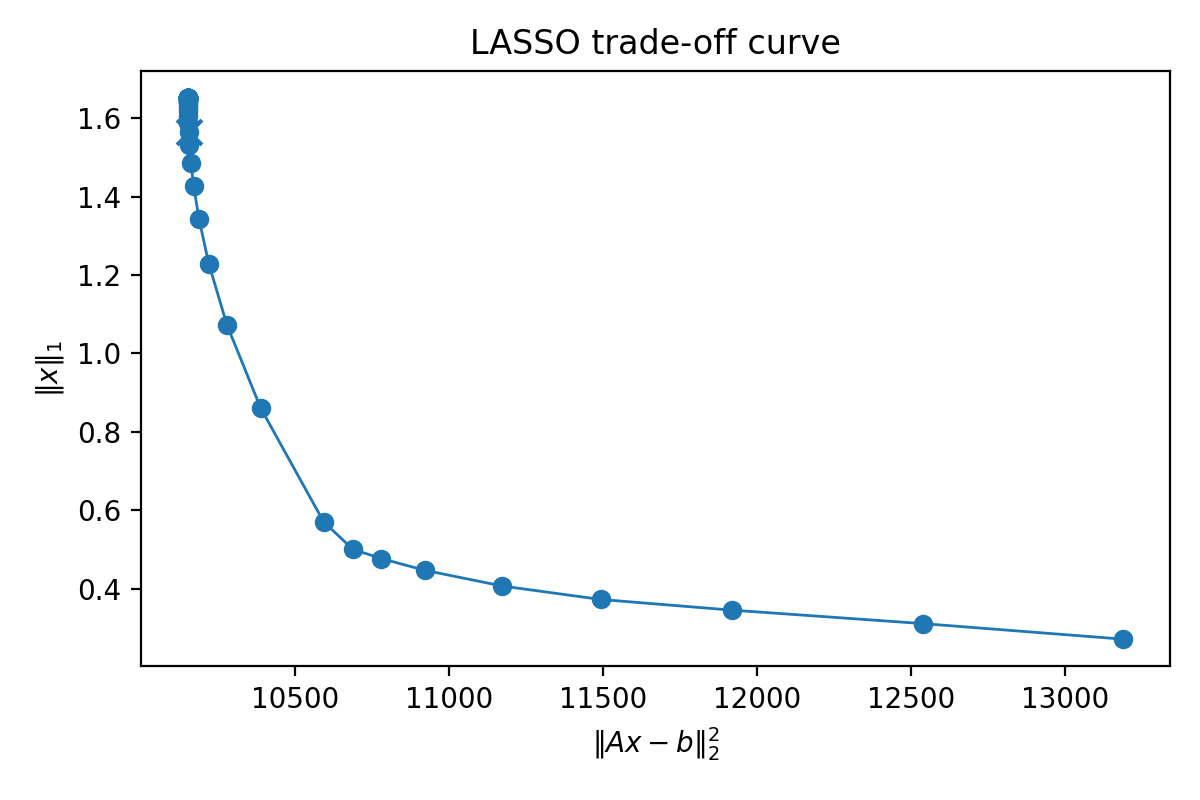
\includegraphics[width=0.62\textwidth]{py/EX_5/results/5_2_lasso_tradeoff.png}
\end{center}

Scripts:
\lstinputlisting{py/EX_5/5_2.py}

\item
For Ridge regression, we solve
\[
\min_x \ \|Ax-b\|_2^2+\lambda\|x\|_2^2
\]
for various choices of \(\lambda\), and plot
\[
\left(\|Ax-b\|_2^2,\ \|x\|_2^2\right).
\]

We again observe a trade-off curve: as \(\lambda\) increases, \(\|x\|_2^2\) decreases, while the training residual \(\|Ax-b\|_2^2\) increases. Compared with LASSO, Ridge shrinks the coefficients more smoothly.

Our selected parameter is
\[
\lambda_{\mathrm{Ridge}} = 0.0001,
\]
and the corresponding solution is
\[
x_{\mathrm{Ridge}} \approx
\begin{bmatrix}
0.510808686\\
0.0156527654\\
-0.180357746\\
0.856848609\\
0.00000700192880\\
-0.00516596448\\
-0.0665626455\\
-0.0172469218
\end{bmatrix}.
\]

Also,
\[
\|x_{\mathrm{Ridge}}\|_2^2 \approx 1.0326437068557672,
\]
\[
\|Ax_{\mathrm{Ridge}}-b\|_2^2 \approx 10151.83179712664,
\]
\[
\|A_{\mathrm{test}}x_{\mathrm{Ridge}}-b_{\mathrm{test}}\|_2^2 \approx 2320.060015006893.
\]

\begin{center}
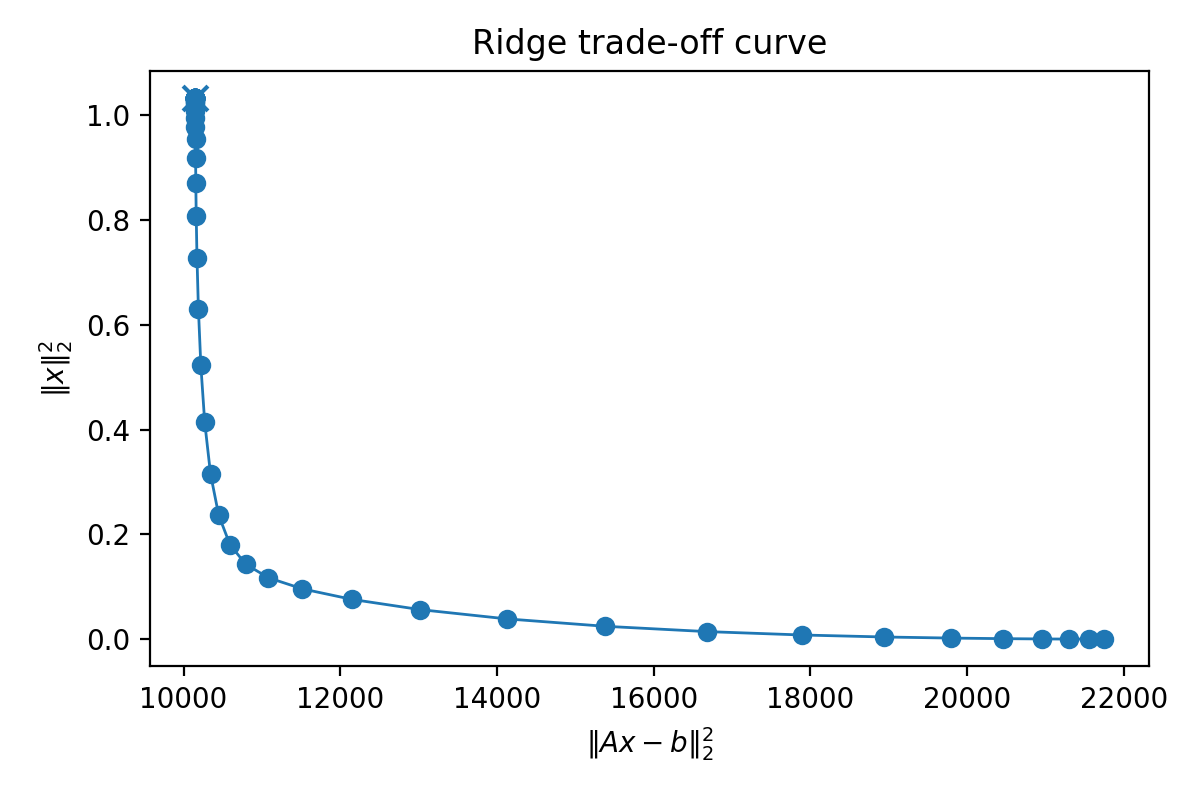
\includegraphics[width=0.62\textwidth]{py/EX_5/results/5_3_ridge_tradeoff.png}
\end{center}

Scripts:
\lstinputlisting{py/EX_5/5_3.py}

\item
The test errors of the three models are
\[
\|A_{\mathrm{test}}x_{\mathrm{LS}}-b_{\mathrm{test}}\|_2^2 \approx 2320.060012898806,
\]
\[
\|A_{\mathrm{test}}x_{\mathrm{LASSO}}-b_{\mathrm{test}}\|_2^2 \approx 2321.052665182842,
\]
\[
\|A_{\mathrm{test}}x_{\mathrm{Ridge}}-b_{\mathrm{test}}\|_2^2 \approx 2320.060015006893.
\]

Hence,
\[
\|A_{\mathrm{test}}x_{\mathrm{LS}}-b_{\mathrm{test}}\|_2^2
<
\|A_{\mathrm{test}}x_{\mathrm{Ridge}}-b_{\mathrm{test}}\|_2^2
<
\|A_{\mathrm{test}}x_{\mathrm{LASSO}}-b_{\mathrm{test}}\|_2^2.
\]

Therefore, among the three models, the least squares solution gives the smallest test error. Ridge regression is almost identical to least squares, since the selected \(\lambda\) is very small. LASSO yields a sparser solution, but its test error is slightly larger in this experiment.

\end{enumerate}

\end{solution}

\newpage
\begin{exercise}
The following problem is for \textit{extra credit}.

Consider the problem of minimizing a convex differentiable function on
\[
\{x \in \mathbb{R}^n \mid x \succeq 0,\; \mathbf{1}^T x = 1\}.
\]

\begin{enumerate}[label=(\alph*)]
    \item Show that the necessary and sufficient condition for optimality is
    \[
    \left\{
    x_i > 0 \;\Longrightarrow\;
    \frac{\partial f}{\partial x_i}
    =
    \min_{j=1,\dots,n}\frac{\partial f}{\partial x_j}
    \right\}
    \cap
    \{x \succeq 0,\; \mathbf{1}^T x = 1\}.
    \]

    \item For the case
    \[
    f(x) := \frac{1}{2}\|x-y\|_2^2
    \]
    (where $y \in \mathbb{R}^n$ is given) derive an efficient algorithm for computing the optimal
    solution and analyze its complexity.

    \item For a randomly chosen $y \in \mathbb{R}^{500}$, solve the problem using your algorithm as
    well as via CVXPY. Compare and explain the implications (please share your results and scripts).
\end{enumerate}
\end{exercise}

\newpage

\begin{solution}

Let
\[
\Delta:=\{x\in\mathbb R^n\mid x\succeq 0,\ \mathbf 1^Tx=1\}.
\]

\begin{enumerate}[label=(\alph*)]

\item
Consider
\[
\min_{x\in\Delta} f(x),
\]
where \(f\) is convex and differentiable.

The Lagrangian is
\[
L(x,\nu,\mu)=f(x)+\nu(\mathbf 1^Tx-1)-\mu^Tx,
\]
where
\[
\mu\succeq 0.
\]
The KKT conditions are
\[
x\succeq 0,\qquad \mathbf 1^Tx=1,\qquad \mu\succeq 0,
\]
\[
\nabla f(x)+\nu \mathbf 1-\mu=0,
\]
\[
\mu_i x_i=0,\qquad i=1,\dots,n.
\]
Since the problem is convex, these conditions are necessary and sufficient.

From
\[
\nabla f(x)+\nu \mathbf 1-\mu=0,
\]
we have
\[
\mu_i=\frac{\partial f}{\partial x_i}+\nu.
\]
Since \(\mu_i\ge 0\),
\[
\frac{\partial f}{\partial x_i}\ge -\nu,\qquad i=1,\dots,n.
\]
If \(x_i>0\), then by complementary slackness,
\[
\mu_i=0,
\]
so
\[
\frac{\partial f}{\partial x_i}=-\nu.
\]
Hence
\[
x_i>0
\quad\Longrightarrow\quad
\frac{\partial f}{\partial x_i}=-\nu.
\]
Since \(\mathbf 1^Tx=1\), at least one component is positive, so
\[
-\nu=\min_{j=1,\dots,n}\frac{\partial f}{\partial x_j}.
\]
Therefore the necessary and sufficient optimality condition is
\[
\left\{
x_i>0
\;\Longrightarrow\;
\frac{\partial f}{\partial x_i}
=
\min_{j=1,\dots,n}\frac{\partial f}{\partial x_j}
\right\}
\cap
\{x\succeq 0,\ \mathbf 1^Tx=1\}.
\]

\item
Now let
\[
f(x)=\frac12\|x-y\|_2^2.
\]
Then
\[
\frac{\partial f}{\partial x_i}=x_i-y_i.
\]
By part (a), at the optimum,
\[
x_i>0
\quad\Longrightarrow\quad
x_i-y_i=\min_j(x_j-y_j).
\]
Equivalently, there exists \(\theta\in\mathbb R\) such that
\[
x_i>0
\quad\Longrightarrow\quad
x_i=y_i-\theta.
\]
Together with \(x_i\ge 0\), this gives
\[
x_i^\star=\max\{y_i-\theta,0\},\qquad i=1,\dots,n,
\]
where \(\theta\) is chosen so that
\[
\sum_{i=1}^n \max\{y_i-\theta,0\}=1.
\]

To compute \(\theta\), sort \(y\) in decreasing order:
\[
u_1\ge u_2\ge \cdots \ge u_n.
\]
Define
\[
\rho
=
\max\left\{
k\in\{1,\dots,n\}\ \middle|\
u_k-\frac{1}{k}\left(\sum_{i=1}^k u_i-1\right)>0
\right\},
\]
and
\[
\theta=\frac{1}{\rho}\left(\sum_{i=1}^{\rho}u_i-1\right).
\]
Then
\[
x_i^\star=\max\{y_i-\theta,0\},\qquad i=1,\dots,n.
\]

The algorithm requires:
\[
\text{sorting: }O(n\log n),
\qquad
\text{prefix sums: }O(n),
\qquad
\text{thresholding: }O(n).
\]
Hence the total complexity is
\[
O(n\log n),
\]
and the memory complexity is
\[
O(n).
\]

\item
We generated a random vector
\[
y\in\mathbb R^{500}
\]
using \texttt{np.random.default\_rng(0).standard\_normal(500)}.

Using the custom projection algorithm, we obtained
\[
\theta = 2.458089440898643,
\]
\[
\text{algorithm\_time} = 0.0009610999841243029,
\]
\[
\frac12\|x_{\mathrm{alg}}-y\|_2^2 = 254.33505541902846.
\]

Using CVXPY, we obtained
\[
\text{cvxpy\_time} = 0.03362550004385412,
\]
\[
\frac12\|x_{\mathrm{cvx}}-y\|_2^2 = 254.3350554190285.
\]

The two solutions agree up to numerical precision:
\[
\|x_{\mathrm{alg}}-x_{\mathrm{cvx}}\|_2
=
8.416972462747517\times 10^{-15},
\]
\[
\|x_{\mathrm{alg}}-x_{\mathrm{cvx}}\|_\infty
=
4.884981308350689\times 10^{-15}.
\]

They also satisfy the simplex constraints numerically:
\[
\mathbf 1^T x_{\mathrm{alg}} = 0.9999999999999996,
\qquad
\mathbf 1^T x_{\mathrm{cvx}} = 0.9999999999999796,
\]
\[
\min_i (x_{\mathrm{alg}})_i = 0,
\qquad
\min_i (x_{\mathrm{cvx}})_i = -1.152064525402398\times 10^{-17}.
\]
Moreover,
\[
|\{i:(x_{\mathrm{alg}})_i>10^{-10}\}|=3,
\qquad
|\{i:(x_{\mathrm{cvx}})_i>10^{-10}\}|=3.
\]

Hence the custom algorithm and CVXPY return essentially the same solution and the same objective value. However, the custom algorithm is much faster:
\[
\frac{\text{cvxpy\_time}}{\text{algorithm\_time}}
\approx 34.99.
\]
Therefore, for this special problem, the explicit simplex projection algorithm is preferable. It exploits the structure of the problem and achieves
\[
O(n\log n)
\]
complexity, while CVXPY incurs additional modeling and solver overhead.

\end{enumerate}

\end{solution}
	
\end{document}
